\documentclass[a4paper, 11pt]{article}

\usepackage{amsmath}
\usepackage{amssymb}
\usepackage{titlesec}
\usepackage[utf8]{inputenc}
\usepackage[margin=2cm]{geometry}
\usepackage{prftree}
\usepackage{changepage}
\usepackage{enumitem}
\usepackage{minted}
\usepackage{lmodern}
\usepackage{graphicx}
\usepackage{wrapfig}

\title{\vspace{-2.5cm}CompArch\vspace{-2cm}}
\author{}
\date{}

\setlength{\parindent}{0cm}
\setlength{\parskip}{2mm}
\setlist{nosep}

% Make ~ look more normal
\let\oldsim\sim
\renewcommand{\sim}{{\oldsim}}

\newmintinline[monospace]{text}{escapeinside=\#\#, mathescape, fontsize=\normalsize}
\newminted[monospacefigure]{text}{frame=lines, framesep=1mm, autogobble, escapeinside=\#\#, mathescape, breaklines}

\titlespacing{\section}{0mm}{2mm}{2mm}
\titlespacing{\subsection}{0mm}{2mm}{2mm}
\titlespacing{\subsubsection}{0mm}{2mm}{2mm}

\begin{document}
\maketitle

Optimisation = Analysis + Transformation

\section*{Unreachable Code Elimination}
{
    \begin{enumerate}
    \item Mark the entry node of each procedure as reachable.
    \item Mark every \textbf{successor} of a marked node, repeat until no change.
    \end{enumerate}

    \texttt{goto} may have multiple potential successor nodes, depending on semantics: jumping to a variable address might mean marking all nodes as reachable.
}
\section*{Unreachable Procedure Elimination}
{
    \begin{enumerate}
    \item Mark \texttt{main} as reachable.
    \item Mark every procedure called from a marked procedure as reachable, repeat until no change.
    \end{enumerate}

    Function pointers (indirect calls) have the same safety issues as \texttt{goto} above. Can improve by only adding functions which are address-taken somewhere in the program, rather than all procedures.
}
\section*{Live Variable Analysis (LVA)}
{
    \begin{itemize}
    \item A variable is \textbf{semantically} live if changing its value affects the \textbf{observable} behaviour of the program.
    \item A variable is \textbf{syntactically} live if there is some path through the flowgraph to a node in which the current value might be \textbf{used} (not necessarily actually hit at runtime).
    \end{itemize}

    Safety constitutes overestimation, that syntactically live variables are a superset of semantically live variables.

    Backwards flow equations. \(\text{def}(n)\) is the set of variable assigned to in the node, \(\text{ref}(n)\) is the set of variables used in the node.
    \begin{align*}
    \text{live}(n) &= \bigg(\bigcup_{s \in \text{succ}(n)}{\text{live}(s)}\bigg) \setminus \text{def}(n) \cup \text{ref}(n) \\\\
    \text{out-live}(n) &= \bigcup_{s \in \text{succ}(n)}{\text{in-live}(s)} \\
    \text{in-live}(n) &= \text{out-live}(n) \setminus \text{def}(n) \cup \text{ref}(n)
    \end{align*}

    For safety with \textbf{pointers}, treat pointer dereferences as referencing any address-taken variable, and assignments to a pointer dereference as not defining any variables: \(\text{ref}(*p) = \{p, x, y, ...\}\) and \(\text{def}(*p = x) = \{\}\).

    \subsection*{Dataflow Anomalies}
    {
        If a variable is live at entry to a procedure, then we can report a warning that a variable has been used before being assigned to.

        Write-write anomalies (writing to a variable without ever reading the old value) can be detected by doing the opposite of LVA: go forwards, and union with \(\text{def}\) instead of \(\text{ref}\) (then each set holds the variables not yet read from). Any instruction which adds an existing variable to the set can be given a write-write anomaly warning.
    }
    \subsection*{Register Allocation by Colouring}
    {
        \begin{itemize}
        \item Generate a graph with virtual registers as nodes and edges between virtual registers which are simultaneously live. Virtual registers represent architectural registers in the IL, but are renamed to physical registers at code generation.
        \item
        {
            Choose a virtual register with the lowest clashes (edges).

            \begin{itemize}
            \item If the number of clashes is lower than the number of colours/physical registers then colour it and remove it from the graph.
            \item Otherwise, mark the register as being spilled to memory (store it in a set) and remove it from the graph.
            \end{itemize}
        }
        \end{itemize}
            
        Spilled registers need relevant \texttt{MOV} instructions to be generated.

        A \textbf{preference graph} can be built up to track extra information about the register dependencies to affect node selection decisions (such as number of accesses, whether the use is in a loop body, programmer \texttt{register} hints, ...).

        \subsubsection*{Spilling}
        {
            We need a spare register to hold variables which were spilled to memory: we may need more if multiple spilled registers are used as operands to the same instruction.

            If we find that we need to spill during register allocation, just restart the register allocation with one register reserved as `temporary' for the spilled value. If we find another spill, reserve another register, and so on (up to the max number of operands per instruction).
        }
        \subsubsection*{Non-orthogonal instructions}
        {
            Instructions that always write to a predetermined register (eg.\ `multiply and store the result in \monospace{r0}') mess up the allocation, as do procedure calls (which use eg.\ registers \monospace{r\{0..4\}} as argument registers and \monospace{r\{5..10\}} as being preserved over function calls).

            \begin{itemize}
            \item Reserve virtual registers for all architectural registers that have special usage (the registers used for results/function arguments).
            \item When an instruction/procedure call requires an operand in an architectural register, generate a preceding \texttt{mov} instruction from the source register to the virtual register (node) which represents the architectural register.
            \item Generate a trailing \texttt{mov} instruction from the virtual register to the destination register for instructions which output to a specific register.
            \end{itemize}

            Remember that the virtual registers \textbf{are} the architectural registers, they represent a logical mapping rather than eg.\ the difference between architectural and physical registers from CompArch. Moving data to the virtual register is just the register-allocation-stage way of moving data to the architectural register: at code generation, we specifically map the reserved arch registers to the real arch registers.
        }
    }
}
\section*{Available Expressions (AVAIL)}
{
    Available Expressions are those expressions that have been syntactically computed prior to that node and haven't been invalidated.

    Forwards flow equations:
    \begin{equation*}
    \text{avail}(n) =
    \begin{cases}
    \bigcap_{p \in \text{pred}(n)}{\big(\text{avail}(p) \setminus \text{kill}(p) \cup \text{gen}(p)\big)} &\text{, if pred}(n) \neq \emptyset \\
    \emptyset &\text{, if pred}(n) = \emptyset
    \end{cases}
    \end{equation*}

    \(\text{gen}(n)\) gives the expressions computed at \(n\), but \textbf{minus any expressions changed by assignments}: \(\text{gen}(\texttt{x = y + z}) = \{\texttt{y + z}\}\), but \(\text{gen}(\texttt{x = x + y}) = \emptyset\), as the new value of \texttt{x} invalidates the expression. \(\text{kill(n)}\) contains the variables assigned to in the node.

    \subsubsection*{Common Subexpression Elimination}
    {
        If an expression is computed both at \(n\) and on a node on all paths to \(n\), then we can arrange for all the prior computations to store their results in a local variable so we don't need to evaluate the expression again.

        \begin{enumerate}
        \item For each node \(n\) containing \monospace{x = a #\(\oplus\)# b} with \monospace{a #\(\oplus\)# b} available at \(n\):
        \item Create a temporary variable \monospace{t} and replace the assignment in \(n\) with \monospace{x = t}.
        \item On each path to \(n\), for the latest computation of \monospace{y = a #\(\oplus\)# b}, add an instruction \monospace{t = y}.
        \end{enumerate}

        Adding an extra variable might make the program worse: it increases register pressure, and memory accesses are often more expensive than the redundant computations.
    }
    \subsection*{Copy Propagation}
    {
        After seeing \monospace{x = y}, replace all subsequent occurrences of \monospace{x} with \monospace{y} (provided \monospace{x} isn't reassigned).

        Can then maybe eliminate the original assignment, which removes a variable so reduces register pressure.

        Useful after CSE, as it can eliminate the temporary variable used.
    }
}
\section*{Static Single Assignment Form (SSA)}
{
    It can be advantageous to use different registers for a variable throughout its scope if it gets reassigned to: otherwise we have a form of false dependency (we depend on the data but are limited by the name).

    SSA uses a new variable for every assignment, which \textbf{minimises the live ranges of each variable}, so allows for \textbf{more efficient register allocation}.

    When paths merge in the flowgraph we need to ensure that temporaries of the same variable which were assigned to on the branches have their values updated into one variable. Can use \(\phi\) functions, which are usually just a theoretical concept: \monospace{x = #\(\phi\)#(x1, x2)} means \monospace{x = x1} if control took a left branch and \monospace{x = x2} if control took a right branch. The \textbf{register allocation pass} can arrange for \monospace{x1} and \monospace{x2} to be assigned to the \textbf{same register}. On some architectures this might not always be possible, so the final resort is to implement an actual branch to update the variables properly.

    Always remember \textbf{live ranges}, they can be great for visualising liveness.
}
\section*{Phase Order}
{
    Different optimisations have different impacts depending on their relative ordering: even preference choices in one pass can alter the effectiveness of subsequent passes. Code motion optimisations are hard to predict the impact of.
}
\section*{Algebraic Identities}
{
    Simple syntax rewriting, replacing eg.\ \monospace{x = 1 + 2} with \monospace{x = 3} or \monospace{[1,2] ++ [3,4]} with \monospace{[1,2,3,4]}.
}
\section*{Strength Reduction}
{
    Generally, switch expensive instructions for cheaper ones. Specifically for loops:

    \begin{enumerate}
    \item Find induction variables which are used as \monospace{i = i #\(\oplus\) c#}.
    \item Find another variable \monospace{j = (i #\(\otimes\)# c1) #\(\oplus\)# c2}.
    \item Move the assigment \monospace{j = (i #\(\otimes\)# c1) #\(\oplus\)# c2} to above the loop.
    \item Add an end-of-loop-body instruction \monospace{j = j #\(\oplus\)# (c1 #\(\otimes\)# c)}.
    \end{enumerate}

    Can then patch up the loop header using the known relation between \monospace{i} and \monospace{j}.

    Example:

    \begin{minipage}[t]{0.45\textwidth}
    \begin{monospacefigure}
    int total = 0;
    for (int x = 0; x < 100; x += 10)
        total += a * x + b;
    \end{monospacefigure}
    \end{minipage}
    \hspace{5mm}
    \begin{minipage}[t]{0.45\textwidth}
    \begin{monospacefigure}
    for (int tot = b; tot < a * 90 + b; )
        tot += 10 * a;
    \end{monospacefigure}
    \end{minipage}
}
\section*{Abstract Interpretation}
{
    Abstract to reach a more easily-computable representation that allows for extracting properties.

    \begin{tabular}{c | c c c}
    \(\otimes\) & \((-)\) & \((0)\) & \((+)\) \\
    \hline
    \((-)\) & \((+)\) & \((0)\) & \((-)\) \\
    \((0)\) & \((0)\) & \((0)\) & \((0)\) \\
    \((+)\) & \((-)\) & \((0)\) & \((+)\)
    \end{tabular}
    \hspace{1cm}
    \begin{tabular}{c | c c c c}
    \(\oplus\) & \((-)\) & \((0)\) & \((+)\) & \((?)\) \\
    \hline
    \((-)\) & \((-)\) & \((-)\) & \((?)\) & \((?)\) \\
    \((0)\) & \((-)\) & \((0)\) & \((+)\) & \((?)\) \\
    \((+)\) & \((?)\) & \((+)\) & \((+)\) & \((?)\) \\
    \((?)\) & \((?)\) & \((?)\) & \((?)\) & \((?)\)
    \end{tabular}

    Abstract interpretations can give different results depending on the syntax, even if the semantics are the same: \((x+1)(x-3)\) has abstract interpretation \((?)\) when \(x = (-)\), but \(x^2 - 2x - 3\) has interpretation \((+)\).
}
\section*{Strictness Analysis}
{
    Use-case of abstract interpretation.

    Associate standard and abstract interpretations with the builtin functions (\(a_i\) and \(a^\sharp_i\)), and deduce standard and abstract interpretations for the user-defined functions (\(f_i\) and \(f^\sharp_i\)).

    Assume the domain of the functions \(D\) is augmented with a value \(\bot\) to represent a non-terminating value: \(D \cup \{\bot\}\).

    A function \(a\) is \textbf{strict} in its \(i\)\textsuperscript{th} parameter iff \(\forall d_i.\; a(d_1, \dots, \bot, \dots, d_n) = \bot\). For example, \(+\) is strict in both parameters as:
    \begin{align*}
    \bot + y &= \bot \\
    x + \bot &= \bot \\
    x + y    &= x +_\mathbb{Z} y
    \end{align*}

    Define the space of abstract values to be \(D = \{0, 1\}\) where \textbf{0 represents guaranteed looping} and \textbf{1 represents possible termination}. Safety here means that we \textbf{underestimate} the strictness of functions (we don't want to alter semantics).

    We can define the abstract interpretations of the builtin functions from their given semantics:
    \begin{equation*}
    a^\sharp(x_1, ..., x_n) = \begin{cases}
        0 & \text{, if }\forall d_i \in D \text{ where }(x_i = 0 \implies d_i = \bot), a(d_1, ..., d_n) = \bot \\
        1 & \text{, otherwise}
    \end{cases}
    \end{equation*}

    The weird condition just means `if \(x_i = 0\) then we force the corresponding semantic argument \(d_i\) to be \(\bot\)'. Essentially just generate \(a^\sharp\) by trying every \(0/1\) input value for the arguments and seeing if \(a\) is terminating or not, then find an expression that matches that. For example, \(x +^\sharp y = x \wedge y\) and \(\text{cond}^\sharp(p, x, y) = p \wedge (x \vee y)\).

    Can generate strictness values for user-defined functions by composing their builtin components. We can't compute it from scratch as it's undecidable (determining whether a functions doesn't terminate): we have to use explicitly specified builtin functions instead.

    In general, need a least-fixed-point iteration over all of the user-defined functions so that updates to one function's strictness predicate updates the predicates of functions that use it. The start value for each strictness predicate should be 0, we assume no functions terminate, then we refine down to more accurate predicates using our knowledge of what definitely terminates.

    \textbf{Example}: \monospace{plus(x, y) = cond(eq(x, 0), y, plus(sub1(x), add1(y)))}.

    Given that \(\text{plus}^\sharp(x,y) = x \wedge y\), \(\text{eq}^\sharp(x,y) = x \wedge y\), \(\text{add1}^\sharp(x) = x\), \(\text{sub1}^\sharp(x) = x\), \(0^\sharp = 1\).
    \begin{enumerate}
    \item \(\text{plus}^\sharp(x, y) = 0\) (initial assumption)
    \item \(\text{plus}^\sharp(x, y) = \text{cond}^\sharp(\text{eq}^\sharp(x,0), y, \text{plus}^\sharp(\text{sub1}^\sharp(x), \text{add1}^\sharp(x))) = x \wedge (y \vee 0) = x \wedge y\)
    \item \(\text{plus}^\sharp(x, y) = \text{cond}^\sharp(\text{eq}^\sharp(x,0), y, \text{plus}^\sharp(\text{sub1}^\sharp(x), \text{add1}^\sharp(x))) = x \wedge (y \vee (x \wedge y)) = x \wedge y\)
    \item No change, so we terminate with \(\text{plus}^\sharp(x,y) = x \wedge y\)
    \end{enumerate}

    The strictness optimisation just allows us to evaluate arguments before passing them as thunk arguments.
}
\section*{Constraint-Based Analysis}
{
    Generally, traverse the syntax tree emitting constraints that are solved later (eg.\ if \monospace{x} is constrained to be even, we can later infer that \monospace{x + 1} is odd).

    \subsubsection*{Control-Flow Analysis}
    {
        Aim to compute the \textbf{set of values} (constants and lambda-abstractions) that any expression in the program can take.

        Language is \(e ::= x \mid c \mid \lambda x.\;e \mid e_1\;e_2 \mid \texttt{let }x = e_1 \texttt{ in } e_2\).

        Define a \textbf{program point} to be a label which uniquely identifies a syntactic expression:\\ \monospace{(let x#\(^2\)# = 1#\(^3\)# in (x#\(^4\)# + 2#\(^5\)#)#\(^6\)#)#\(^1\)#}.

        Associate a \textbf{flow variable} (representing the set of possible values) with each program point (\(\alpha_1\), ...)/ The space of possible \textbf{flow values} for the example above are \(\{\texttt{1}^3, \texttt{2}^5, \texttt{(x}^4\texttt{ + 2}^5\texttt{)}^6\}\).

        Safety consists of overestimating the possible values computed by the expressions.

        \begin{itemize}
        \item For a term \(x^i\), generate \(\alpha_i \supseteq \alpha_j\) where \(\alpha_j\) is the flow variable for the expression bound to \(x^i\) (eg.\ by \((\lambda x^i.\;...)\;e^j\) or \(\texttt{let }x^i\texttt{ = }e^j\texttt{ in }...\)). Don't think this is actually necessary as \(\alpha_i\) should be constrained by the bindings themselves.
        \item For a term \(c^i\), generate \(\alpha_i \supseteq \{c^i\}\).
        \item For a term \((\lambda x^j.\;e^k)^i\), generate \(\alpha_i \supseteq \{(\lambda x^j.\;e^k)^i\}\).
        \item For a term \((e_1^j\;e_2^k)^i\), generate \((\alpha_k \rightarrow \alpha_i) \supseteq \alpha_j\).
        \item For a term \((\texttt{let }x^l\texttt{ = }e^j\texttt{ in }e^k)^i\), generate \(\alpha_i \supseteq \alpha_k\) and \(\alpha_l \supseteq \alpha_j\).
        \item For a term \((\texttt{if }e_1^j\texttt{ then }e_2^k\texttt{ else }e_3^l)^i\), generate \(\alpha_i \supseteq \alpha_k\) and \(\alpha_i \supseteq \alpha_k\).
        \end{itemize}

        \((\alpha_k \rightarrow \alpha_i) \supseteq \alpha_j\) is shorthand for `whenever \((\lambda x^a.\;e^b)^c \in \alpha_j\) then \(\alpha_a \supseteq \alpha_k\) and \(\alpha_i \supseteq \alpha_b\)'. This means that \textbf{any of the actual parameters become possible values of the formal parameters, and the possible values of the application are the possible values of the function bodies}.

        This approach is monovariant (0-CFA), which imposes the inaccuracy that different invocations of a function all affect the same set of possible values, rather than just a call-site specific version. A polyvariant approach fixes this.
    }
}
\section*{Inference-Based Program Analysis}
{
    Generally, use a judgement system like \(\Gamma\vdash e : \phi\) to infer properties from the terms of the language. Type systems are a specific example, but can be generalised:
    \begin{align*}
    & \Gamma = \{2 : \text{even}, (+) : (\text{even}\rightarrow\text{even}\rightarrow\text{even}) \wedge (\text{even}\rightarrow\text{odd}\rightarrow\text{odd}) \wedge ..., (\times) : ...\} \\
    & \Gamma\vdash (\lambda x.\;\lambda y.\;2 \times x + y) : ...
    \end{align*}

    \subsection*{Effect Systems}
    {
        Specific example of inference-based program analysis, modelling communicating systems.

        Model effects as \(W_C\) and \(R_C\) for write/reads to a channel \(C\), use terms \(C!e_1.\;e_2\) for writing \(e_1\) and \(C?x.\;e\) for reading \(x\).

        Judgements of the form \(\Gamma\vdash e : t, F\), with immediate effects \(F\). Latent effects are reresented by tags on function types, \(t_1 \stackrel{F}{\rightarrow} t_2\).

        \begin{gather*}
        \prftree[r]{(var)}
        {x:t \in \Gamma}
        {\Gamma\vdash x : t,\emptyset}
        \qquad
        \prftree[r]{(abs)}
        {\Gamma,x:t_1\vdash e : t_2,F}
        {\Gamma\vdash (\lambda x.\;e) : t_1 \stackrel{F}{\rightarrow} t_2,\emptyset}
        \qquad
        \prftree[r]{(app)}
        {\Gamma\vdash e_1 : t_1 \stackrel{F_l}{\rightarrow} t_2}
        {\Gamma\vdash e_2 : t_1, F_2}
        {\Gamma\vdash e_1\;e_2 : t_2, F_1 \cup F_2 \cup F_l}
        \\
        \\
        \prftree[r]{(read)}
        {\Gamma,x:\text{int}\vdash e : t, F}
        {\Gamma\vdash (C?x.\;e) : t, F \cup \{R_C\}}
        \qquad
        \prftree[r]{(write)}
        {\Gamma\vdash e_1 : \text{int}, F_1}
        {\Gamma\vdash e_2 : t, F_2}
        {\Gamma\vdash (C!e_1.\;e_2) : t, F_1 \cup F_2 \cup \{W_C\}}
        \\
        \\
        \prftree[r]{(sub)}
        {\Gamma\vdash e : t_1 \stackrel{F_l}{\rightarrow} t_2, F}
        {F_l \subseteq F_l'}
        {\Gamma\vdash e : t_1 \stackrel{F_l'}{\rightarrow} t_2, F}
        \end{gather*}

        The \(\text{sub}\) rule is necessary to patch-up the types when there's eg.\ a conditional expression where the two branches are functions with different latent effects.

        Can change the representation of effects to carry more information: allow writing values of types other than \(\text{int}\), or use lists instead of sets to capture ordering information.
    }
}
\section*{Alias Analysis (Andersen's Analysis)}
{
    Similar to 0-CFA. Given a pointer \(p\), find the \textbf{locations} that it might point to \(\text{pt}(p)\).

    \begin{itemize}
    \item For a term \(x := \texttt{null}\), generate \(\text{pt}(x) \supseteq \{\texttt{null}\}\).
    \item For a term \(x := \&y\), generate \(\text{pt}(x) \supseteq \{y\}\).
    \item For a term \(x := \texttt{new}_l\), generate \(\text{pt}(x) \supseteq \{\texttt{new}_l\}\).
    \item For a term \(x := y\), generate \(\text{pt}(x) \supseteq \text{pt}(y)\).
    \item For a term \(x := *y\), generate \(\text{pt}(x) \supseteq \text{pt}(z)\) for all \(z \in \text{pt}(y)\).
    \item For a term \(*x := y\), generate \(\text{pt}(z) \supseteq \text{pt}(y)\) for all \(z \in \text{pt}(x)\).
    \end{itemize}

    Most important thing to remember is that \(\text{pt}(x)\) is the set of \textbf{locations} that \(x\) can point to, not the values. Then the rules aren't hard to reproduce.

    If \(\text{pt}(x) \cap \text{pt}(y) = \emptyset\) then \(x\) and \(y\) cannot point to the same location, so we can reorder assignments or perform parallelisation etc.

    Safety is that \(\text{pt}(x)\) is an overapproximation of the true pointers that can be pointed to.
}
\section*{Instruction Scheduling}
{
    Instruction dependencies prevent instruction reordering:
    \begin{itemize}
    \item Read after Write
    \item Write after Read
    \item Write after Write
    \end{itemize}

    Instruction scheduling aims to minimise the number of pipeline stalls or bubbles, or increase the program ILP, \textbf{while preserving the dependencies} to ensure program semantics. No dynamic reordering of loads before stores at runtime like a processor can do.

    \begin{enumerate}
    \item Construct a scheduling DAG for each basic block, with nodes being instructions. Scan backwards through the block and add a dependency edge from \(a\) to \(b\) if \(a\) occurs before \(b\) in the original order and cannot be moved before it.
    \item
    {
        Considering just the minimal elements (lowest in-degree) of the DAG:
        \begin{itemize}
        \item Emit an instruction satisfying the static scheduling heuristics.
        \item If no instruction satisfies the heuristics then emit a NOP.
        \item Remove the instruction from the DAG.
        \end{itemize}
    }
    \end{enumerate}

    The static scheduling heuristics are:
    \begin{itemize}
    \item Choose an instruction not conflicting with the previous emitted instruction (as that would introduce a stall).
    \item Choose an instruction most likely to conflict if first of a pair (eg.\ load before add as loads conflict with most instructions whereas adds conflict with few).
    \item Choose an instruction as far as possible (along paths in the DAG) from a maximal instruction (highest in-degree).
    \end{itemize}

    \begin{minipage}[t]{0.3\textwidth}
    Original:
    \vspace{-5mm}
    \begin{monospacefigure}
    1: LD   r1  0(r0)
    2: LD   r2  4(r0)
    3: ADD  r3  r1      r2
    4: ST   r3  12(r0)
    5: LD   r4  8(r0)
    6: ADD  r3  r1      r4
    7: ST   r3  16(r0)
    \end{monospacefigure}
    \end{minipage}
    \hspace{1mm}
    \begin{minipage}[t]{0.2\textwidth}
    \vspace{0pt}
    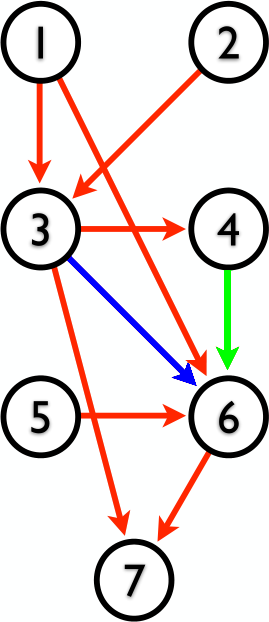
\includegraphics[width=\textwidth]{dependency-graph.png}
    \end{minipage}
    \hspace{3mm}
    \begin{minipage}[t]{0.45\textwidth}
    Reordered:
    \vspace{-5mm}
    \begin{monospacefigure}
    1: minimal node, tie break randomly
    2: minimal node, tie break randomly
    5: minimal node, 3 conflicts with 2
    3: minimal node, no tie break
    4: minimal node, no tie break
    6: minimal node, no tie break
    7: minimal node, no tie break
    \end{monospacefigure}
    \end{minipage}

    When making a dependency graph, remember to check \textbf{every pair of nodes} for \textbf{all 3 dependency types}.

    In the original code, there are \textbf{stalls} between lines 2-3 and 5-6 as the data we need isn't available yet. In the reordered code, there are no stalls.

    Assume that loads take eg.\ 1 cycle to complete, so any instruction needing the loaded data conflicts.
}
\section*{Decompilation}
{
    Legality: sketchy, get a lawyer or do it on own code.

    Compilation isn't injective, so can't perfectly recover source code. Optimisations further obfuscate original structure as they rearrange things at a low level.

    To recover structural information we extract a flowgraph of basic blocks from the machine code then match them against standard structures from the source language (loops, if statements etc).

    In a flowgraph, node \(m\) \textbf{dominates} node \(n\) if control \textbf{has} to go through \(m\) to reach \(n\) (there are no paths to \(n\) which don't go through \(n\)). \textbf{Strict domination} further implies that \(m \neq n\). The \textbf{immediate dominator} of \(n\) is the unique node that strictly dominates \(n\) but doesn't dominate any other strict dominator of \(n\). This isn't as simple as `immediate parent' or similar.

    The \textbf{dominance frontier} of \(m\) is the set of nodes \(n\) such that \(m\) doesn't dominate \(n\) but does dominate an immediate predecessor of \(n\): the set of nodes `where \(m\)'s dominance no longer holds'.

    A \textbf{dominance tree} is a tree (independent of the flowgraph) with nodes being basic blocks and an edge between two nodes if the parent is the immediate dominator of the child.

    A \textbf{back edge} \(b \rightarrow a\) in the dominance graph is an edge where the head also dominates the tail (\(a\) also dominates \(b\), although probably not directly). Every back edge has an associated loop, where the head \(a\) is the loop header and the loop body is \textbf{all the nodes that can reach \(b\) without passing through the header \(a\)}.

    \begin{minipage}[t]{0.47\textwidth}
    \centering
    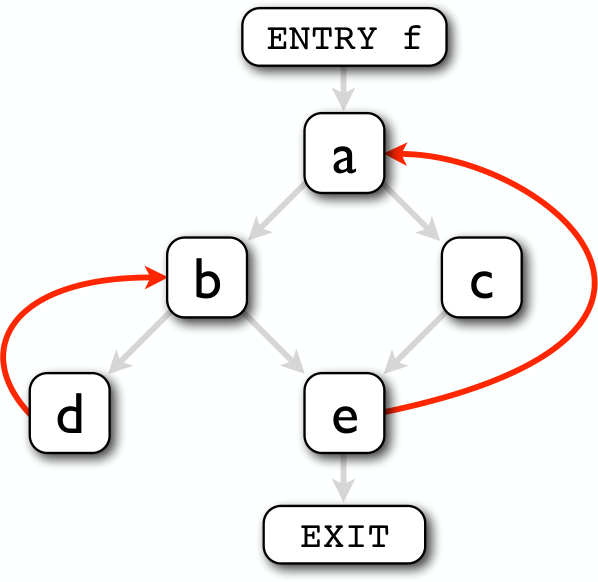
\includegraphics[height=7cm]{flow-graph.png}

    \textbf{Flowgraph with dominance edges}

    Back edges are in red, dominating predecessors in grey.
    \end{minipage}
    \hspace{5mm}
    \begin{minipage}[t]{0.47\textwidth}
    \centering
    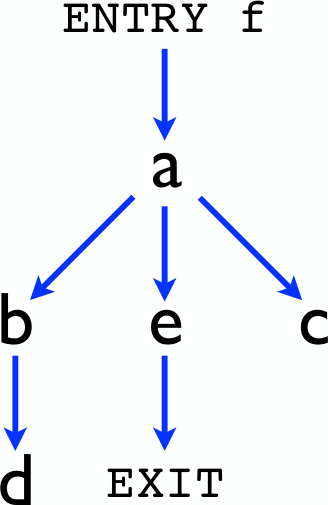
\includegraphics[height=7cm]{dominator-tree.png}

    \textbf{Dominance tree}

    Immediate dominators of each node: \(a\) is the immediate dominator of \(e\) as neither \(b\) nor \(c\) dominate \(e\) (they aren't on the only path to \(e\)). Both \(a\) and \texttt{ENTRY} are strict dominators of \(e\), but \texttt{ENTRY} can't be the immediate dominator as it dominates \(a\).
    \end{minipage}

    \begin{minipage}[t]{0.47\textwidth}
    \vspace{10mm}
    \(b\) and \(a\) are loop headers, as they have a back-edge going into them.
    
    \begin{itemize}
    \item The loop body for \(b\) is just \(d\), as we can get from \(d\) to \(d\) trivially but can't reach any other nodes without going through \(b\).
    \item The loop body for \(a\) is every other node except \texttt{ENTRY} and \texttt{EXIT}, as we can \textbf{reach \(e\) from all of them without passing through \(a\)}. Note that without the back-edge from \(d\) to \(b\), \(d\) wouldn't be included as it can't reach \(e\).
    \end{itemize}

    \vspace{3mm}

    The \textbf{type of loop} can be detected from the flowgraph structure: \(b\) either allows executing the body \(d\) or moving immediately to \(e\) so is a \texttt{while} loop, but in contrast \(a\) unconditionally executes the body (no other outgoing edges), so is a \texttt{do while} loop.

    \vspace{3mm}

    Conditionals are either \texttt{if x then y} or \texttt{if x then y else z}: the structure can also be detected from the flowgraph. Conditionals have the common structure that they always end up at the same block.
    \end{minipage}
    \hspace{5mm}
    \begin{minipage}[t]{0.47\textwidth}
    \vspace{0pt}
    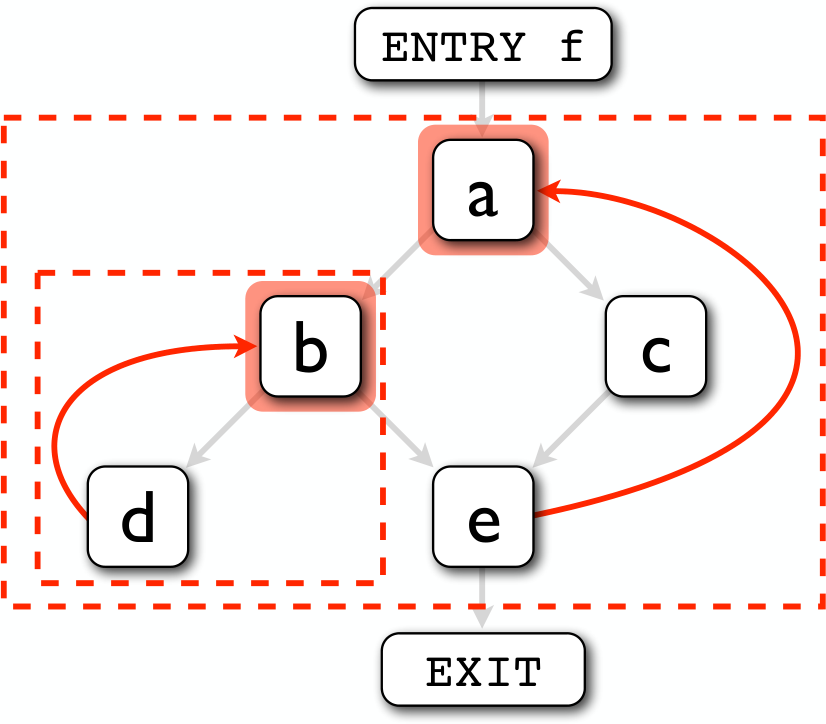
\includegraphics[width=\textwidth]{loops.png}

    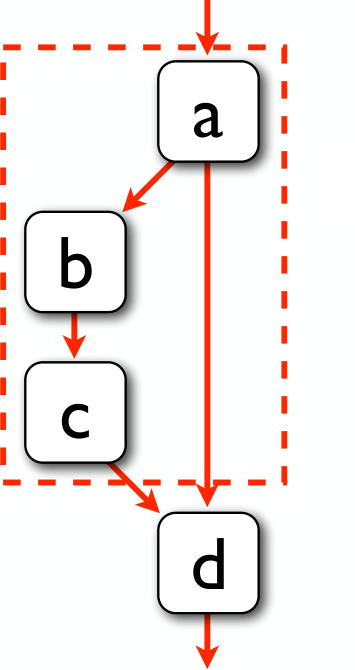
\includegraphics[width=0.4\textwidth]{if.png}
    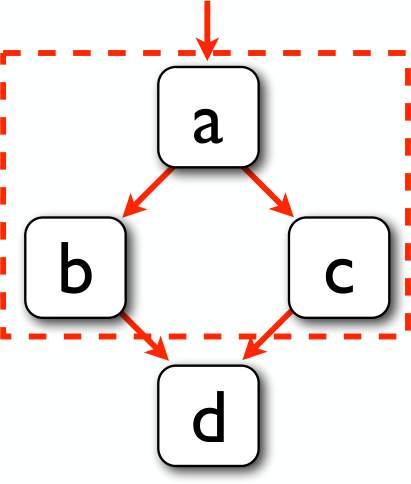
\includegraphics[width=0.4\textwidth]{ifelse.png}
    \end{minipage}

    \subsection*{Type Reconstruction}
    {
        
    }
}
\end{document}